\section{Soll-Zustand}
Der Ist-Zustand im vorigen Kapitel hat gezeigt, dass viele manuelle Tätigkeiten für die Beladung und Abfertigung sowie die Rangiervorgänge von Güterwagen im Einzelwagenverkehr notwendig sind.\par
Dies verursacht hohe Kosten durch die benötigte Zeit (siehe dazu auch den Zeitvergleich in Abbildung \ref{fig:Zeitvergleich} auf Seite \pageref{fig:Zeitvergleich}) und das benötigte Personal, sowie auch Kosten an der Verladestelle, wenn diese aufgrund von Kupplungs- und Rangiervorgängen still steht.\par
Bei einem Umbau für die Demonstratoren muss darauf geachtet werden, dass ein voll- ständiger Rückbau der neuen Einrichtungen möglich ist, aber auch so bahntauglich ist, dass die Demonstratoren für ein Folgeprojekt oder Feldversuche genutzt werden können. Diese Projekt muss nicht sofort zulassungsfähig sein, sollte aber eine Basis dazu bilden. \par
An der Bewegung der Wagen im Wagenverband an sich mit Hilfe einer Lok oder eines anderen Rangierhilfsmittel soll hier nichts automatisiert werden. Siehe dazu auch Kapitel \ref{sec:Zustellfahrt}, \ref{sec:Zugfahrt} und \ref{sec:Rangierfahrt}. Automatisierungen können und sollen aber selbst verständlich im Bereich der Kupplung, Bremse oder auch der informationstechnischen Prozesse stattfinden.\par
Zur besseren Einordnung sollen nun diese Komponenten definiert und erläutert werden aus denen sich verschiedene Stufen ergeben und aus denen sich wiederum später verschiedene Anforderungen ergeben.

\subsection{Bremse}
Die Einführung einer automatischen Bremse soll vor allem zur Zeitersparnis bei der Zugvorbereitung und Bremsprobe führen.\par
Besonders wichtig zur Einführung der automatisierten Bremse ist die Fernbetätigung dieser. Sie sollte vorallem die Möglichkeiten zum Schnelllösen, aus- und einschalten der Bremse, Änderung der Bremsstellung und Einstellen der Feststellbremse (auch automatische Parkbremse) haben.
Durch ein TSI-konformes Steuerventil soll die Umstellung der Bremsarten mittels G/P-Umsteller automatisiert werden. Auch eine automatische Lastabbremsung mittels Wiegeventil ist vorgesehen. Hier ist bei beiden Funktionen vor allem auf eine sichere Funktion und Rückmeldung zu achten.
Für diese sichere Übertragung ist die Messung des C-Drucks von größter Wichtigkeit.
Auch fernbetätigte Absperrhähne sollen zu dieser Zeiteinsparung führen. 
Da der Zustand der Bremse nicht mehr zwangsläufig von außen sichtbar ist, ist eine Bremszustandsanzeige am Wagen anzubringen. 
Durch eine Automatisierung der Bremse ist nun auch eine ep-Bremsung möglich.

\subsubsection{Fernbetätigung Bremse}
Die Fernbetätigung der Bremse soll vorallem die Zeit des entlanglaufen des Zuges beim Prüfen der Bremse ersparen. Es müssen folgende Funktionen fernbetätigt werden können:
\begin{itemize}
    \item Schnelllösen
    \begin{itemize}
        \item Ein Löseimpuls löst die Schnelllösefunktion des Steuerventils aus.
        \item Der Löseimpuls kann elektromechanisch oder pneumatisch auf das Steuerventil übertragen werden.
    \end{itemize}
    \item Bremse aus
    \begin{itemize}
        \item Die Funktion ist bistabil umzusetzen.
        \item 	Es werden folgende Verbindungen geöffnet bzw. geschlossen:
        \begin{itemize}
            \item HLL - SV (Entlüftung zum SV)
            \item SV - R (Entlüftung zum SV)
            \item SV - Cv (Entlüftung zum Relaisventil)
        \end{itemize}
        \item Die Betätigung muss in weniger als 10 Sekunden durchgeführt werden.
    \end{itemize}
    \item Bremsstellung
    \begin{itemize}
        \item Die Bremsstellung wird elektrisch bistabil durch Verstellen des SV umgestellt.
        \item Eine Rückmeldung ist vorzusehen.
    \end{itemize}
    \item Festellbremse
    \begin{itemize}
        \item Die Feststellbremse kann unabhängig von der pneumatischen Energie im Wagen angelegt und gelöst werden.
        \item Das Anlegen und Lösen erfolgt bistabil durch eletrischen Impuls.
        \item Eine Rückmeldefunktion für den gelösten Zustand ist vorzusehen.
        \item Die Bremskraft am Bremszylinder beträgt ??kN (für 2\%-Gefälle, 90 t, Klotzbremse).
        \item Alternative Lösungen, wie Federspeicher oder FT Park Lock können vorgeschlagen werden
        \item mit Luft = ungebremst, ohne Luft = gebremst
    \end{itemize}
\end{itemize}

\subsubsection{Steuerventil}
Die Bremsarten G und P sollen mittels Aktor sicher umgestellt und detektiert werden. Auch eine Übertragung der aktuellen Stellung soll sicher gemeldet werden. Aus Zulassungsgründen soll ein UIC/TSI-kompatibels Steuerventil eingesetzt werden. Dieses verfügt dann über die Bremsstellungen G und P, über automatisches Schnelllösen. \par
Ein zusätzliches Relaisventil ist für die automatische Lastabbremsung mittels Wiegeventil vorgesehen. Dieses ist vorzugsweise nicht im Steuerventil integriert.

\subsubsection{Messung C-Druck}
Der Bremszylinderdruck (D-Cruck) wird gemessen. 
%2.	Der Sensor arbeitet als Stromsensor (4-20 mA).
%3.	Der Messbereich ist (0...5) bar.
Die Messunsicherheit und Auflösing ist so gewählt, dass die erste und letzte Bremsstufe %(0,45 bar Cv) 
sicher erkannt werden. %Eine Messunsicherheit von 0,05 bar erfüllt diese Anforderung.

\subsubsection{Fernbetätigte Absperrhähne}
Die Endabsperrhähne sind bistabil, d.h. verbleiben ohne Betätigung in ihrem letzten Zustand. Ein freier Querschnitt von 1,25'' wird für sinnhaft erachtet. Die Betätigungszeit für den Übergang Öffnen-Schließen beträgt maximal 60 s. Die Hähne sind von ihrem Funktionsprinzip für Anforderungen nach DIN EN 14601 geeignet, diese muss allerdings noch nicht von Demonstratoren und Labormuster erfüllt sein. Eine fahrzeugseitige Verschraubung nach G1 1$/$4i (DIN EN ISO 228-1) ist zu bevorzugen. Für den Demonstrator kann die Kompatibilität durch einen Adapter hergestellt werden. Kupplungsseitig ist eine Verschraubung mit Whitworth-Gewinde mit stumpfen Gewinden für G1 1$⁄$4i—Leitungen zu bevorzugen. Für den Demonstrator kann die Kompatibilität durch einen Adapter hergestellt werden.

\subsubsection{Zustandsanzeige Bremse}
\begin{figure}[htbp]
    \centering
    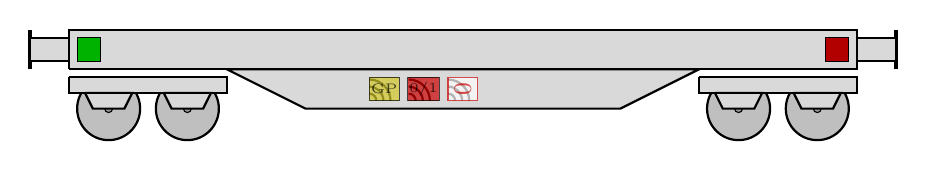
\begin{tikzpicture}[font = \sffamily]
%        \node (a) at (0,0) {};
%        \node (b) at (6,0) {};
        \draw[fill = gray!30, thick] (0,3) -- (10,3) -- (10,3.5) -- (0,3.5) -- (0,3);
        \draw[fill = gray!30, thick] (2,3) -- (3,2.5) -- (7,2.5) -- (8,3) -- (2,3);
        %DG 1
        \draw[fill = gray!50, thick] (8.5, 2.5) circle[radius = .4cm];
        \draw[fill = gray!80] (8.5, 2.5) circle[radius = .05cm];
        \draw[fill = gray!50, thick] (9.5, 2.5) circle[radius = .4cm];
        \draw[fill = gray!80] (9.5, 2.5) circle[radius = .05cm];
			\draw[fill = gray!30, thick] (8,2.9) -- (10,2.9) -- (10,2.7) -- (8,2.7) -- (8,2.9);
			\draw[fill = gray!30, thick] (8.2,2.7) -- (8.3,2.5) -- (8.7,2.5) -- (8.8,2.7) -- (8.2,2.7);
			\draw[fill = gray!30, thick] (9.2,2.7) -- (9.3,2.5) -- (9.7,2.5) -- (9.8,2.7) -- (9.2,2.7);
        %DG 2
        \draw[fill = gray!50, thick] (0.5, 2.5) circle[radius = .4cm];
        \draw[fill = gray!80] (0.5, 2.5) circle[radius = .05cm];
        \draw[fill = gray!50, thick] (1.5, 2.5) circle[radius = .4cm];
        \draw[fill = gray!80] (1.5, 2.5) circle[radius = .05cm];
			\draw[fill = gray!30, thick] (0,2.9) -- (2,2.9) -- (2,2.7) -- (0,2.7) -- (0,2.9);
			\draw[fill = gray!30, thick] (0.2,2.7) -- (0.3,2.5) -- (0.7,2.5) -- (0.8,2.7) -- (0.2,2.7);
			\draw[fill = gray!30, thick] (1.2,2.7) -- (1.3,2.5) -- (1.7,2.5) -- (1.8,2.7) -- (1.2,2.7);
	%Puffer 2
			\draw[ultra thick] (10.5,3) -- (10.5, 3.5);
			\draw[fill = gray!30, thick] (10.5,3.1) -- (10,3.1) -- (10,3.4) -- (10.5,3.4) -- (10.5,3.1);
	%Puffer 2
			\draw[ultra thick] (-.5,3) -- (-.5, 3.5);
	 		\draw[fill = gray!30, thick] (-.5,3.1) -- (0,3.1) -- (0,3.4) -- (-.5,3.4) -- (-.5,3.1);
			% Neues UIC-Zeichen
			%\node [cloud, cloud puffs=9, draw = none, fill = yellow!80!black, minimum width=.8cm, minimum height=.3cm, font = \tiny, inner sep = 0] at (4, 3.25) {4.0};
			% Aussenanzeigen
			\draw[fill = green!70!black] (0.1,3.1) -- (0.4,3.1) -- (0.4,3.4) -- (0.1,3.4) -- (0.1,3.1);
			\draw[fill = red!70!black] (9.9,3.1) -- (9.6,3.1) -- (9.6,3.4) -- (9.9,3.4) -- (9.9,3.1);
			%\node[draw, fill = white, font = \small, inner sep = 0.6, minimum height = 0.3cm] at (4, 3.25) {P 86};
			\draw[thick] (3.90, 2.6) arc (0:90:.09cm);
			\draw[thick] (3.99, 2.6) arc (0:90:.18cm);
			\draw[thick] (4.08, 2.6) arc (0:90:.27cm);
			\node[opacity = .7, draw, fill = yellow!80!black, font = \tiny, inner sep = 0.6, minimum height = 0.3cm, minimum width = 0.38cm] at (4, 2.75) {GP};
			\draw[thick] (4.40, 2.6) arc (0:90:.09cm);
			\draw[thick] (4.49, 2.6) arc (0:90:.18cm);
			\draw[thick] (4.58, 2.6) arc (0:90:.27cm);
			\node[opacity = 0.7, draw, fill = red!80!black, font = \tiny, inner sep = 0.6, minimum height = 0.3cm, minimum width = 0.38cm] at (4.5, 2.75) {0/1};
			\draw[thick] (4.90, 2.6) arc (0:90:.09cm);
			\draw[thick] (4.99, 2.6) arc (0:90:.18cm);
			\draw[thick] (5.08, 2.6) arc (0:90:.27cm);
			\node[opacity = 0.7, draw = red!80!black, text = red!80!black, fill = white, font = \small, inner sep = 0.6, minimum height = 0.38cm, minimum width = 0.3cm, rotate = 90] at (5, 2.75) {0};

\end{tikzpicture}

    \caption{Zustandsanzeige Bremse \cite{ETR_3}}
    \label{fig:ZustandBremse}
\end{figure} 
Da der Zustand der Bremse nicht mehr zwangsläufig von außen sichtbar ist, siehe dazu Abbildung \ref{fig:ZustandBremse}, ist eine Bremszustandsanzeige am Wagen anzubringen. Hier ist mindestens eine Anzeige je Fahrzeugende zum Einbau am Pufferträger ist vorzusehen, so dass
 der Zustand der Bremse im Drehgestell immer zu erkennen ist. Die Anzeige stellt den Zustand der Bremskupplung (drucklos/druckbeaufschlagt) dar. Die Anzeige muss Überdrücke %> 0,5 bar 
 in den Bremskupplungen anzeigen, bspw. durch die Farbe "Rot'' im Schauglas. Bei Unterschreiten des Drucks wird bspw. die Farbe "Grün'' angezeigt. Die Anzeige muss auch im stromlosen Zustand verfügbar sein.

\subsubsection{ep-Bremse}
Das ep-Brems-Ventil wird mit der HLL verbunden und zum Bremsen bestromt. Das Ventil entlüftet die HLL im Wagen in (3,5...5) s von Regelbetriebsdruck auf 3,5 bar.

\subsection{Kupplung}
Wie in Kapitel \ref{sec:Personal} angedeutet und in Kapitel \ref{sec:LuftumechKup} beschrieben, ist das mechanische Kuppeln und das Kuppeln von Luft aufwändig, körperlich anstrengend und fehlerbehaftet. \par
Zur Automatisierung von mechanischen Kupplungen gibt es Kupplungsrobotoren\footnote{Zum Beispiel die Bahn-Kupplungs-Robotoren BaKuRo und EntKuRo}, dort muss aber weiter händisch Luft gekuppelt werden \textbf{Ist das so?}. Alternativ ist die Automatische Kupplung eine Lösung, aber auch nach deren Einführung im vorigen Jahrhundert ist eine flächendeckende Nutzung im Güterverkehr noch nicht realisiert.\par
\textbf{Irgendwas zu Luft und elektrischen Ventilen.}\\
\textit{siehe auch \ref{sec:Vorpruefung} und \ref{sec:Zugvorbereitung}}
\par
Aufgrund dieser Punkte ist es erst einmal sinnvoll mich der mechanischen Kupplung weiter zu machen und Lösungen für die Automatische Kupplung kompatibel zu halten. Vor allem muss aber die Luftkupplung vereinfacht wreden wo es geht \textbf{ SIEHE AUCH: Luftventile.}

\subsection{Bewegung des Wagens}
In Kapitel \ref{sec:BewdWagen} werden die verschiedenen Möglichkeiten der Wagenbewegung betrachtet. Im Allgemeinen werden dafür zusätzliche Fahrzeuge, Personal und eine Gleisanlage benötigt. Je nach Beschaffung der Gleisanlage und die in Kapitel \ref{sec:Fahrweg} angesprochene Einschränkung, werden zusätzliche Sägefahrten zur korrekten Einsortierung der Wagen auf verschiedene Gleise benötigt. \par
Ein eigener Antrieb auf jedem Wagen, der eine selbstständige Bewegung in geringer Geschwindigkeit zulässt wäre hier eine Lösung.\par
\textit{\textbf{Probleme:} Stromversorgung, Akkuaufladung, Antrieb, Sicherheit}
\subsubsection{Adrücken}
DAs Abdrücken am Ablaufberg, siehe Kapitel \ref{sec:Abdruecken} ist bereits auf großen Rangierbahnhöfen automatisiert, siehe Kapitel \ref{sec:automAbdruecken}, dennoch ist auch dies Handarbeit zur Vorbereitung. Die Wagen müssen vorentkuppelt werden, sowohl mit der Luftkupplung, als auch mechanisch, dann aber wieder, mit einem Hemmschuh, festgelegt werden und kurz vorm Ablaufberg vollständig entkuppelt. 
Hemmschuh, vereinzeln, vorentkuppelt, Geschwindigkeit
\subsection{Sicherheit/Zugintegrität}
\subsubsection{Personalschulung}
Neue Systeme benötigen immer Zeit zur Einführung und Schulung des Personlas. Das gilt auch für dieses Projekt, aber auch jetzt schon sind die Handgriffe, wie in Kapitel \ref{sec:Personal} angesprochen, kompliziert und fehleranfällig. Durch informationstechnische Prozesse \textbf{MEHR DAZU UNTER}, die zusätzlich im Hintergrund laufen und durch weniger Handgriffe im üblichen Betrieb, sollen diese Prozesse einfacher und sicherer werden. Zusätzlich sollen die neu benötigten Handgriffe intuitiv zu den alten Handgriffen passen oder leicht erlenrnbar sein. Zusätzliches Schulungsmaterial soll leicht verständlich und intuitiv gestaltet werden.\par
\textit{\textbf{Probleme:} Annahme der Systeme, Kosten für die Schulung}

\subsection{Informationstechnische Prozesse}
1.	Alle elektrischen Komponenten arbeiten mit 24 V.
\subsubsection{Bremshundertstel/Bremsberechnung}
Die Bremshundertstel werden bisher, genau wie das Bremsgewicht, händisch mittels Bremszettel berechnet. \textbf{BILD}. Auf diesem Vordruck trägt der Triebfahrzeugführer Achszahl, Zugmasse und Bremsgewichte des Zuges ein. Daraus berechnen sich die Bremshundertstel. Nach Vergleich dieser mit den Mindest-Bremshundertstel der Strecke, ergibt sich Höchstgeschwindigkeit und Bremsstellung. die Bremsstellung wird nach jeder neuen Zusammenstellung und vor Fahrtantritt, siehe Kapitel \ref{sec:UEdWagen}, neu berechnet.\par
Diese manuelle Berechnung ist für Triebfahrzeugführer tägliche Arbeit, dennnoch ist sie Fehleranfällig und kann durch Rechnereinsatz einfach automatisiert werden.
\subsubsection{Bremsprobe}
\textbf{SIL-Bewertung - liegt nicht an, liegt an, sicheres lösen, sicheres stellen}.\par
Die \gls{Bremsprobe} findet zur Vorbereitung einer Sperr-, Rangier- oder Zugfahrt statt und überprüft die Funktionsfähigkeit des Bremssystems im Zug- oder Wagenverbund.\par
\begin{figure}[htbp] 
    \begin{center}
            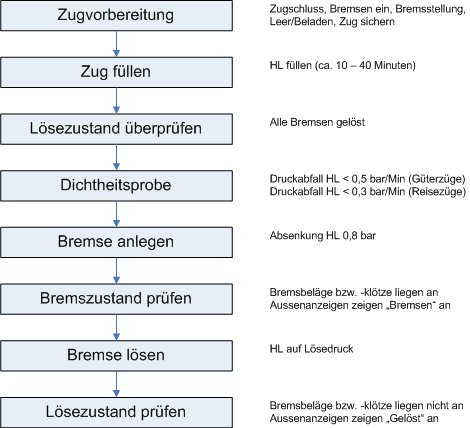
\includegraphics[width=9cm]{Bilder/bremsprobe.png}
            \caption{Schematische Übersicht der Bremsprobe}
            \label{fig:Bremsprobe}
    \end{center}
\end{figure} 
Sie wird von Bremsprobeberechtigten nach genau vorgeschriebenem Ablauf durchgeführt. Ja nach Zustand des Zuges und Fälligkeit der \gls{Bremsprobe} wird eine volle, vereinfachte, stationäre oder Führerraumbremsprobe durchgeführt. Der genaue Ablauf ist in der \acrshort{RIL} 915 oder der VDV-Schrift 757 geregelt und als grobe Übersicht in Abbildung \ref{fig:Bremsprobe} zu sehen.\par
\textit{Durch bekannte Vorprüfungen kann die vollständige \gls{Bremsprobe} vereinfacht werden. Zum Beispiel durch sogenannte vorgeprüfte Gruppen.\\
\textbf{Siehe auch DI, Luftventile\\
\ref{sec:vBremsprobe}, \ref{sec:UEdWagen}, \ref{sec:RangKnoten}}}
\textbf{Siehe auch Bremsprobe im Anhang}
\subsubsection{technische Wagenbehandlung}
Es gibt vier Stufen der technischen Wagenbehandlung. Diese sind der RIL 936 definiert.
\begin{itemize}
    \item TWb Stufe 1: Behandlung vor einer Rangierfahrt
    \item TWb Stufe 2: Prüfung nach Abstellung (PnA)
    \item TWb Stufe 3: Prüfung vor Zugfahrt
    \item TWb Stufe 4: Untersuchung und Qualitätscheck der Wagen
\end{itemize}
Siehe dazu auch Anhang \ref{sec:ATWb}.\par
\textbf{Durch Rechnereinsatz kann Stufe X vereinfacht werden zu ... trotzdem langlaufen?}
\subsubsection{Transportdokumente}
Wie bereits In Kapitel \ref{sec:Transdoc} beschrieben, gibt es die papierlose Transportabwicklung inklusive Gefahrgutdokumenten bisher im LKW-Bereich, allerdings nciht im Bahnsektor. Ein Grund dafür ist die fehlende Dateninfrastruktur.\par
Durch eine durchgängige Stromversorgung auf dem Wagen und einen bahntauglichen Rechner sowie entsprechende Datenverbindungen kann dieses Problem angegangen werden.\par
\textit{\textbf{Siehe dazu auch:} Stromversorgung, Rechner, Datenverbindung, DI (Digitale Identität)}
\subsubsection{Vergleicher}
\ref{sec:Vorpruefung}
\subsubsection{Zugvorbereitung}
\ref{sec:Vorpruefung}